\documentclass[french]{article}

\usepackage{graphicx}

\title{\Huge Génération automatique de modèles de test pour la validation des DSL}

\author{Soilihi Ben Soilihi Boina}

\date{14/12/2019}

\begin{document}


\includegraphics{images/logo_udem.png}

\maketitle

\newpage

\textbf{Abstract :}

\parindent=1cm
\par
\hspace{10 mm} 
 L'avancée de jour en jour à pas géants des technologies et l'ampleur que cela prend de plus en plus, notamment avec le développement d'internet, des applications autogérées, l'utilisation d'environnements de plus en plus variés et contraints (terminaux mobiles, automobiles, robots...) et dans des contextes de plus en plus critiques (aérospatial, médical, militaire, nucléaire) ont considérablement complexifié le développement des systèmes informatiques.
\par 
Avec toutes ces complexités et ses importances, il est nécessaire, voire primordial de valider la fonctionnalité du logiciel pour le rendre fiable en effectuant des tests. Le test de logiciel est une discipline intensément étudiée et différentes techniques, dont les plus utilisées, comme le test de mutation demandent une génération automatique de données de test. 
\par
Notre travail consiste à justement générer ces données de test qui seront traduits par un ensemble de modèles aléatoires diversifiés générés. Notre solution a été développé dans Eclipse Epsilon avec EOL et notre approche se base sur les objets du modèles pour en générer les instances.

\newpage

\section{Introduction :}
		
\hspace{10 mm} Les outils DSL(Domain Specific Language) devenant de plus en plus complexes à implémenter avec toutes les spécifications et les fonctionnalités pointues suivant l'avancement technologique, ainsi que l'importance qu'ils occupent dans de nombreuses disciplines qui sont assez critiques requièrent une certaine confiance des utilisateurs. Pour ce faire, il nous doit de faire des tests pour nous assurer qu'ils fonctionnents correctement. 
			\par 
			L'un des tests les plus utilisés et fiable est le test de mutation qui consiste à ajouter des erreurs que seraient susceptibles de commettre le développeur ou d'autres pour s'assurer que le programme est capable de les détecter et les gérer. Ce dernier se divise en certaines étapes dont l'une, et la plus crucial est la prise en charge d'un jeu de tests et des mutants pour pour les exécuter et comparer les sorties. Le jeu de tests requiet un ensemble de modèles diversifiés et plus les modèles sont nombreux et divers, plus le test de mutation est efficace. 
			 \par
			 Le projet consiste justement à faire une transformation pour générer automatiquement des modèles diversifiés aléatoirement qui peuvent être ensuite utilisés pour faire un test qui demande un certain nombre de modèles distincts comme le test de mutation.
		 
		 Nous verrons dans l'article la présentation du projet et l'outil utilisé puis l'implémentation suite à quoi nous concluerons avant de voir les travaux futurs et perspectives.	

\newpage
	 	
		
\section{Présentation du projet et outil :}
\subsection{Présentation du projet :}

\hspace{10 mm} Une DSL est essentiellement composé d'une syntaxe abstraite et d'une syntaxe concrète. La syntaxe abstraite constitue le coeur du programme et ainsi, quand elle est correcte, tout le reste l'est souvent. C'est pour cela que pour vérifier des DSL, les efforts seront mis dans la vérification de celle ci vu qu'elle implique souvent l'autre.
	\par Notre transformation doit prendre un métamodèle et générer des modèles d'instances à partir du métamodèles. Les modèles doivent être différents, conformes au métamodèle et être générés d'une façon automatique et aléatoires. Ici, on a utilisé le métamodèle de MindMap et on générera des instances à partir de ça. Mais le processus peut être utilisé pour généraliser ça avec n'importe quel diagramme de classe et nous donnerons plus de détails dans les perspectives.\\
	 Ci-dessous une image de ce métamodèle.
	
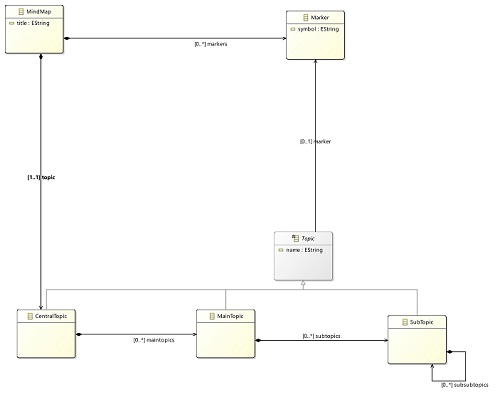
\includegraphics{images/MindMap.jpg}	
\newpage
\subsection{Outil :}

	\hspace{10 mm} Notre solution agit sur les objets constituant un modèle Ecore représentant un diagramme de classe. Donc on a utilisé le langage des objets d'Epsilon (EOL). EOL est utilisé comme un langage de gestion de modèle autonome à usage général pour automatiser des tâches. Il est organisé par modules qui eux-mêmes sont composé de corps et d'opérations. Le corps est un bloc d'instructions qui sont évaluées lorsque le module est exécuté et les opérations définissent chacune le type d'objets sur lesquels elles sont applicables. [1]\\
	
Ci-dessous une image qui présente le fonctionnement d'EOL :
\flushleft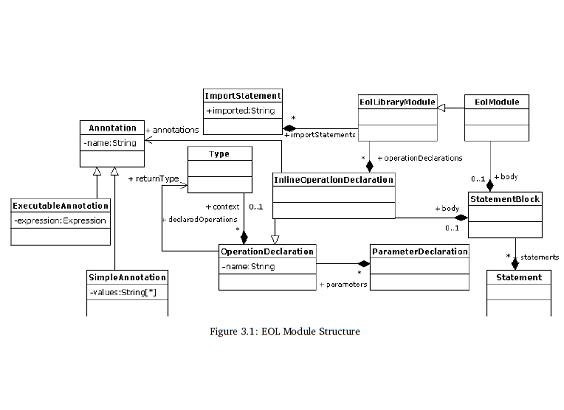
\includegraphics{images/eol.png}

\newpage
	
\section{Implémentation :}
\subsection{construction :}
\hspace{10 mm} Comme on disait, EOL est composé de modules, chaque modules représente un fichier avec l'extention ".eol". Il agit sur un modèle Ecore pour y faire les transformations. Dans notre cas, il va agir sur un fichier le modèle "MindMap.ecore". La liaison se fait à la configuration, en utilisation le même nom du modèle que celui du fichier .eol. 
\par
Les étapes, c'est qu'on crée un modèle Ecore à partir duquel on peut générer ou non un fichier ".emf" (Emphatic Source) puis en suite, on écrit nos instructions dans le fichier ".eol" pour la transformation.

\subsubsection{Création du modèle Ecore :}
\hspace{10 mm} On ouvre Epsilon puis on crée un nouveau projet général:\linebreak \\ 

\hspace{13 mm} \textit{File--New--Other--General--Project--(Give a name)--Finish} \linebreak \\ 
Dedans, on crée un fichier Ecore et pour cela, on fait : \linebreak 
\hspace{13 mm} \textit{File--New--Other--Ecore file--(Give a name)--Finish} \linebreak \\
Ensuite, on il faut construire le fichier Ecore, à savoir reproduire le métamodèle de mindmap soit dans le modèle Ecore lui-même, soit graphiquement avec une représentation comme un diagramme de classe UML et pour cela, on fait : \linebreak \\ 
\textit{Right click on Ecore--Initialise Ecore Diagram--(Give a name)--Next--Finish} \linebreak \\

\subsubsection{Création du fichier eol :}
\hspace{13 mm} \textit{File--New--Other--Eol program--(Give a name)--Finish}  \linebreak \\
C'est ici qu'on va écrire notre transformation.

\newpage

\subsection{Configuration et execution :}

\textit{Go to run button--click on the arrow--Run new configurations...--} \linebreak \\

Une nouvelle fenêtre s'ouvre dans laquelle il faut chercher notre fichier ".eol" et cliquer dessus.
Suite à ça, on passe à la partie droite composé de 5 onglets : Source, Models, Parameters, Profiling, Common.
\par
Dans source, on clique sur \textit{BrowseWorkSpace} et on met notre fichier ".eol". \\
On passe à l'onglet suivant, à savoir "models".
On clique sur \textit{Add} et donne un nom. \linebreak \\
\textbf{Attention :} le nom qu'on donne ici doit être le même que celui qu'on utilisera pour créer un nouvel objet du métamodèle dans le fichier eol.\\
Ensuite, on rajoute le métamodèle de mindmap dans la partie métamodèle, puis, on a qu'à appliquer et exécuter le programme.

P.S : pour la première exécution, il faut décocher la case "Read on load".

\newpage

\section{Conclusion et perspective :}
	
	Notre transformation prend en entrée un métamodèle mindmap et génère des sorties multiples dynamiques de modèles mindmap. Ces modèles peuvent être utilisés dans un jeu de test d'un test de mutation.
	\par 
	Le même processus peut-être utilisé pour généraliser ça avec n'importe quel type de métamodèle. Pour cela, il faudrait essayer le même procédé sur plusieurs autres métamodèles et essayer de voir les choses qui changent et ceux qui se repètent pour ainsi ressortir une manière uniforme pour n'importe quel métamodèle. Une perspéctive serait de trouver un moyen d'avoir des modèles logiques en excluant les modèles répétitifs ou équivalents, ainsi que les mutants équivalents pour ainsi améliorer au maximum la qualité du jeu de test et ainsi du résultat du test de mutation. 		

\newpage
\section{Reférences :}	
1. \textbf{The Epsilon Book} \linebreak
\textit{Dimitris Kolovos, Louis Rose, Antonio García-Domínguez, Richard Paige}\linebreak
Last update: July 29, 2018.\linebreak \\
2. \textbf{Iterative Generation of Diverse Models
for Testing Specifications of DSL Tools} \linebreak
\textit{Oszkar Semerath1 and Daniel Varro1}\linebreak \\
3.\textbf{Génération automatique de modèles de
test pour les transformations de modèles
en exploitant l’analyse de mutation} \linebreak
\textit{Thomas Degueule} \linebreak \\
4. \textbf{Une approche déclarative pour la génération de modèles} \linebreak
   \textit{Adel Ferdjoukh}\linebreak \\

\textbf{Website : } \linebreak \\
1. https://www.eclipse.org/epsilon/doc/eol/ \linebreak \\

2.https://www.eclipse.org/epsilon/examples/index.php?example=org.eclipse.epsilon.examples.buildooinstance \linebreak \\

3. La chaine youtube \textbf{Epsilon Devs}

\end{document}